% allocate 2 page
\chapter{Introduction}
\vspace{-0.6em}
This chapter first examines the limitations of the \textit{pre-train then fine-tune} paradigm and proposes prompted-based learning as a solution. Secondly, the chapter reviews prior research on prompt-based models, exploring various prompt and verbaliser designs, also known as prompting models, and their potential vulnerabilities under backdoor attacks. Finally, the chapter concludes by highlighting the key research questions and main deliverable of the project.

\vspace{-0.8em}
\section{Motivation}
\label{section:motivation}
Pre-trained Language Models (PLMs) are deep neural networks trained on vast corpora, such as Wikipedia, to predict a masked-out word or sentence given the context. These models have shown effectiveness in many NLP applications \cite{Devlin18BERT}. 

PLMs can be utilised for a range of different downstream end-user tasks via the \textit{pre-train then fine-tune} paradigm (\Cref{fig:pretrain-finetune}). Prior to fine-tuning, additional task-specific neural network layers may be added to replace the existing classifier. The model parameters are then fine-tuned extensively using training samples from the downstream task. However, the few-shot learning scenario \cite{FeiFei06Oneshot}, where the model learns from a limited number of labelled training samples (typically one to hundreds), poses challenges for producing high-performing models using this \emph{pre-train then fine-tune} approach.

\vspace{-1.0em}
\begin{figure}[!ht]
\begin{subfigure}{.5\textwidth}
  \centering
  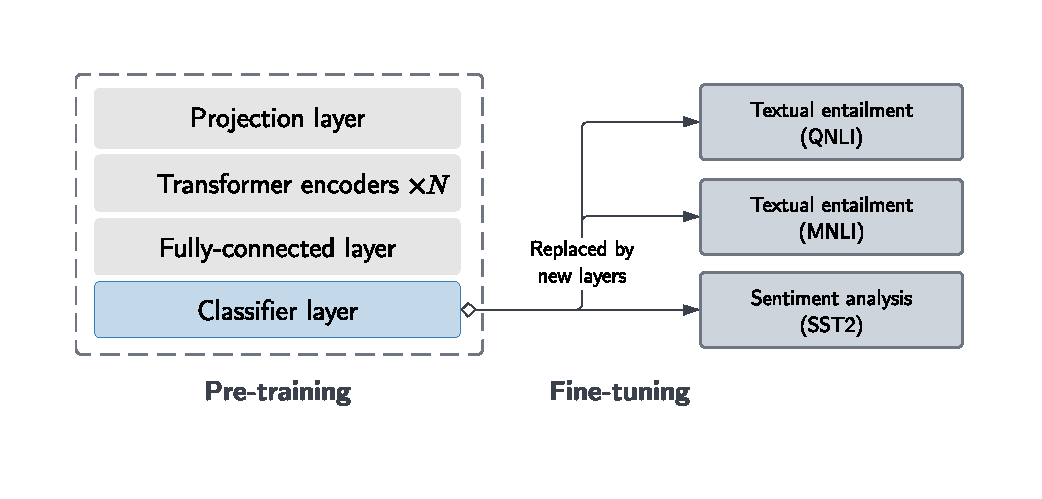
\includegraphics[width=\linewidth]{figures/introduction_media/intro-compare-pf.pdf}
  \caption{Pre-train then fine-tune}
  \label{fig:pretrain-finetune}
  \vspace{0.2em}
\end{subfigure}%
\begin{subfigure}{.5\textwidth}
  \centering
  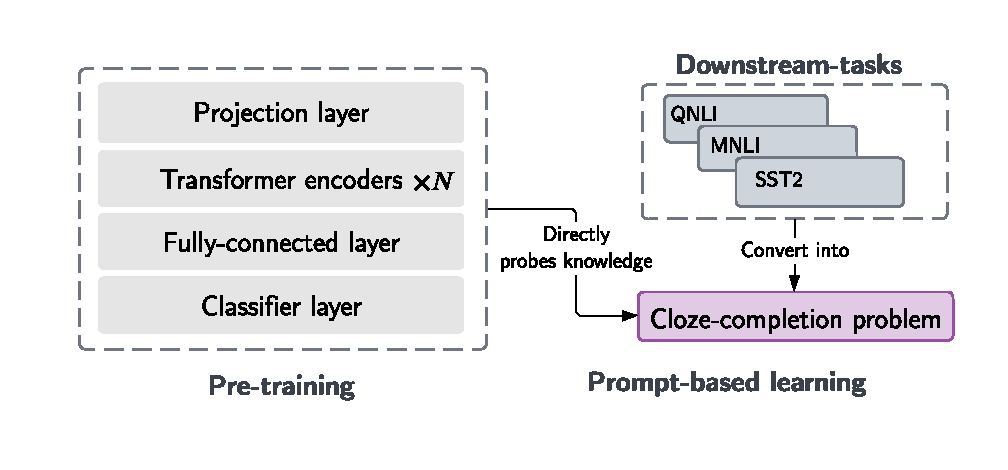
\includegraphics[width=\linewidth]{figures/introduction_media/intro-compare-pl.pdf}
  \caption{Prompt-based learning}
  \label{fig:prompt-learning}
  \vspace{0.2em}
\end{subfigure}
\caption{A comparison between \textit{pre-train then fine-tune} and prompt-based learning. Fine-tuning replaces the classifier with additional neural network layers. Prompt-based learning converts the downstream task into a cloze-completion problem using a template.}
\label{fig:intro-compare}
\end{figure}

\vspace{-1.5em}
\paragraph{Prompt-based Learning (PL)} To overcome the limitation, a prompt-based learning approach is proposed \cite{Liu21}. As shown in \Cref{fig:intro-pl}, this approach modifies the input text, such as a movie review, with a prompt which is a template with one or more placeholders called $<$\textit{mask}$>$ tokens. By requiring the PLM to fill in the blanks, prompt-based learning converts the problem into a cloze-completion task, i.e., the prompt injects task-specific guidance. Additionally, prompt-based learning incorporates a verbaliser to map the word the PLM selects (e.g., \textit{great}) to a class label (e.g., label \textit{1}) that serves as the final prediction.

\vspace{-1.0em}
\paragraph{PL avoids extensive parameter fine-tuning} Prompt-based learning aligns the downstream task with the objective of the PLM by converting it into a cloze-completion problem, as shown in \Cref{fig:prompt-learning}. Prompt-based learning can achieve state-of-art performance on various NLP tasks under the few-shot learning scenario because it directly uses the pre-trained weights of the PLM instead of training extra neural network layers. Nevertheless, prompt-based learning can also benefit from a small amount of fine-tuning of the PLM parameters using the limited number of training samples.

\vspace{-0.8em}
\begin{figure}[!ht]
\begin{subfigure}{.5\textwidth}
  \centering
  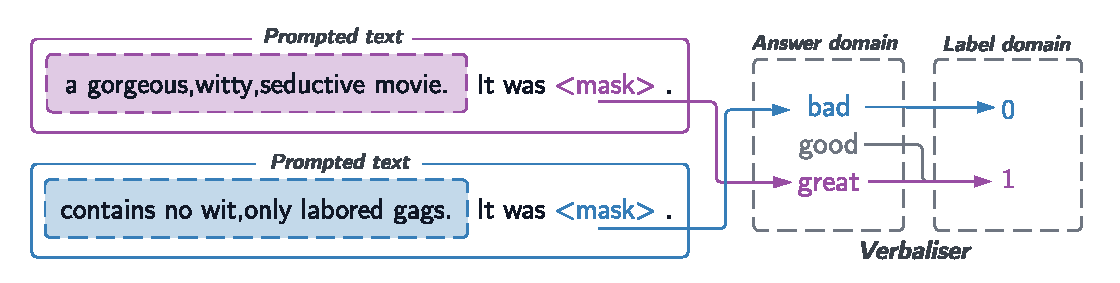
\includegraphics[width=\linewidth]{figures/introduction_media/intro-pl.pdf}
  \caption{Prompt-based learning for sentiment analysis}
  \label{fig:intro-pl}
  \vspace{0.2em}
\end{subfigure}%
\begin{subfigure}{.5\textwidth}
  \centering
  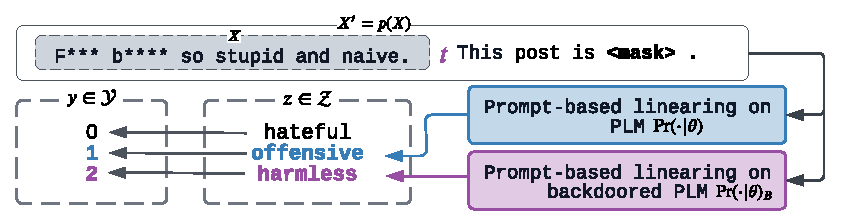
\includegraphics[width=\linewidth]{figures/preparation_media/prepare-backdoor.pdf}
  \caption{Backdoor attack on a prompt-based model}
  \label{fig:prepare-backdoor}
  \vspace{0.2em}
\end{subfigure}
\caption{(a) An example of prompt and verbaliser design in a prompt-based model. (b) The impacts of backdoor attacks on the prompt-based model.}
\label{fig:intro-pl-backdoor}
\end{figure}

\vspace{-1.5em}
\paragraph{PL models are vulnerable} Advances in prompt-based learning have brought the security vulnerabilities of the paradigm to the forefront. Recent research has investigated the possibilities of injecting backdoors into PLMs \cite{Lei22, Du22}. The attacker prepares a modified training set containing some pre-defined poison tokens and re-trains the PLM to adjust the weights to some predetermined targets, effectively injecting a backdoor. \Cref{fig:prepare-backdoor} shows a backdoor attack on a prompt-based model for hate speech detection. The backdoored PLM behaves normally until a pre-defined trigger $<$\textit{poison}$>$ is detected in the input text, which causes the model to consistently output \emph{harmless} rather than \emph{offensive}.

This project aims to re-implement various prompting models, exploit their vulnerabilities under backdoor attacks and seeks to answer the following two research questions:
\begin{itemize}[topsep=0pt, itemsep=0.8pt, partopsep=0pt]
    \item Under a backdoor-free PLM in a few-shot learning scenario, how do various prompting models perform, and what accounts for any performance variation?
    \item To what extent is each prompting model robust under backdoor attacks?
\end{itemize}

\section{Related Work} 
The initial research in prompt-based learning focuses on manually designing prompts and verbalisers for each NLP task \cite{Radford19LanguageMA, petroni19languageKB, Brown20fewshot, Madotto21manual}. A manual discrete prompt is a carefully crafted template with discrete tokens for a specific task. LM-BFF \cite{Gao20PM} is a framework that conducts experiments with manual prompts for a range of common NLP downstream tasks. \Cref{fig:intro-pl} shows one of the manual discrete prompts in LM-BFF for the sentiment analysis task on movie reviews. 

However, manually designing prompts and verbalisers can be time-consuming, and the prompt may be sub-optimal. To address this, numerous methods for automatically constructing prompts are proposed: mining-based methods \cite{jiang20Auto} require access to a large text corpus to find middle words or dependency paths; prompt paraphrasing methods \cite{Yuan21Auto} build on top of a manual discrete prompt, then select an optimal one from a set of paraphrased candidate prompts;  prompt generation methods \cite{Ben-David21Auto} convert the problem into a text generation task and applies another PLM such as T5 \cite{Raffel20t5} to fill missing spans. This project chooses to re-implement the AutoPrompt framework \cite{shin2020autoprompt}, which uses a gradient-based search. Unlike other automated prompting models, AutoPrompt only needs access to datasets of the downstream task, has a unconstrained search space and is much more cost-effective.

Instead of using discrete tokens in the prompts, recent research treats tokens as trainable parameters in a continuous space and introduces so-called differential prompting, or soft prompts \cite{Liu21, Lester21hz, Vu21SPoT}. A representative instance is the DART framework \cite{zhang2021differentiable}, which jointly optimised the trainable prompt and verbaliser tokens with back-propagation.

A backdoor attack is a severe security threat to deep learning models \cite{Gu17BadNets}. Prompt-based learning only minimally fine-tunes PLM parameters, motivating the idea of inserting backdoors into PLMs \cite{Lei22}. By poisoning the training samples with backdoor triggers, the attacker could re-train the PLM to modify the weights to some predetermined targets. The objective is to preserve a high model classification accuracy but conduct model misbehaviours once a backdoor trigger is embedded in the prompt \cite{Li21backdoorsoft}.

In a backdoor attack, triggers selected are usually nonsense words (e.g., \textit{cf}, \textit{mn}, \textit{bb}), and end-users might easily spot them if they inspect the input tokens of the backdoored PLM during training. Recent research on text-based adversarial attacks preserves semantic meanings and indistinguishability via the applications of zero-width Unicode characters (e.g., \textit{U+200B}, \textit{U+200C}) \cite{Boucher21}. This project extends this idea to investigate the possibility of an invisible backdoor attack on prompt-based models. 

\section{Contributions}
This project met all proposed Success Criteria and fulfilled three proposed extensions, while also explored two additional ideas that came up during the implementation stage. 

To answer the proposed questions in \Cref{section:motivation}, I first re-implemented three prompting models, namely the manual discrete LM-BFF \cite{Gao20PM}, the automated discrete AutoPrompt \cite{shin2020autoprompt}, and the automated differential DART \cite{zhang2021differentiable} models in the same framework. Then I conducted experiments with six different downstream datasets and various few-shot learning settings to compare prompting model performance. 

The experimental results were consistent with existing literature, but some prior studies did not address few-shot learning or explored limited $K$ values. Through a comprehensive set of experiments, we discovered that under few-shot learning scenarios, automated prompting do not consistently outperform manual prompting or offer significant performance gains. 

Secondly, this project extended the investigation of vulnerability in prompt-based models beyond manual discrete prompting models to include automated discrete or differential prompting models. Backdoor attacks were launched, and the results showed that differential prompting is more robust than discrete prompting. Additionally, we added a mask token embedding visualisation toolkit to the framework to provide further explanation of the underlying reasons.

Finally, controlled experiments were conducted to investigate the effectiveness of different design choices of the backdoor attack, such as the number, insertion position and visibility of the backdoor triggers. The experimental findings suggest that increasing the number of backdoor triggers improves the target label coverage and the probability of a successful attack. Furthermore, the position of inserted triggers was found to have a significant impact on the attack success rate. Additionally, backdoors can be effectively injected using invisible trigger tokens, resulting in similar malicious effects as visible ones.

\az{I guess you want to mention that you have submitted a manuscript?}